

\documentclass[10pt]{article}
\usepackage{tikz}
\usepackage{listings}
\usepackage[english]{babel}
\usepackage[autostyle]{csquotes}


\author{Andrew}
\date{text }

\begin{document}
\begin{center}
CPSC 413 Assignment 1 \\
by Andrew Garcia-Colrey
\end{center}
\part{Mailmen Problem}
Question 1
\begin{center}
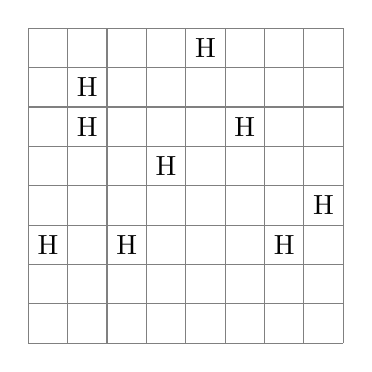
\begin{tikzpicture}
\draw[step=0.5cm,color=gray] (-1,-1) grid (3,3);
\node at (1.25,+2.75) {H};
\node at (-.25,+2.25) {H};
\node at (-0.25,+1.75) {H};
\node at (+0.75,+1.25) {H};
\node at (1.75,+1.75) {H};
\node at (2.75,+0.75) {H};
\node at (+2.25,0.25) {H};
\node at (+.25,+0.25) {H};
\node at (-.75,.25) {H};
\end{tikzpicture}
\end{center}
Question 2
\hfill \break
\break
Two ways to look at this problem is to either minimize the amount of houses that are visited, or to maximize the amount of house each Mailmen finds. In my search for an algorithm I began debating between two main Algorithms I will refer to as \textbf{Shortest}  and \textbf{Most Houses}. 
\hfill \break
\break
\textbf{Shortest} simply starts by looking both down and right and checks to see from the current position of the mailman which one is closer and takes a step in that direction. then proceeds to checks again by looking down and to the right to see if there is a house closer to himself now that he has moved in on of the two directions.
\hfill \break
\break
 \textbf{Most Houses} works in a similar fashion the previous Algorithm by looking in both directions. However where this Algorithm differ is that instead of looking for closest House, it instead looks for the most amount of Houses in that direction regardless of how far away it is. then upon moving in the direction with the most houses, the Algorithm then repeats the previous check by looking in both directions to ensure that.
 \hfill \break
\break
However upon further examination and counter example exploration the  \textbf{Most Houses} fails to give an optimal solution for the following graph

\noindent\fboxsep{%
\begin{minipage}{14em}
 \centering
 Figure 1 \textbf{Shortest}
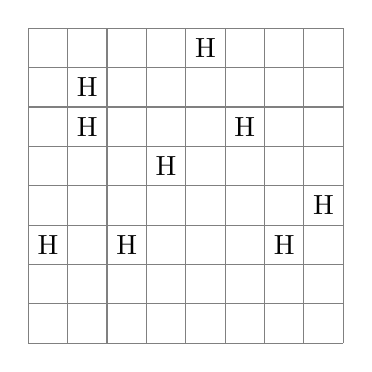
\begin{tikzpicture}

\draw[step=0.5cm,color=gray] (-1,-1) grid (3,3);
\node at (1.25,+2.75) {H};
\node at (-.25,+2.25) {H};
\node at (-0.25,+1.75) {H};
\node at (+0.75,+1.25) {H};
\node at (1.75,+1.75) {H};
\node at (2.75,+0.75) {H};
\node at (+2.25,0.25) {H};
\node at (+.25,+0.25) {H};
\node at (-.75,.25) {H};
\end{tikzpicture}
\end{minipage}}%
\hfill%
\fboxsep{%
\begin{minipage}{14em}
 \centering
 Figure 2 \textbf{Most Houses}
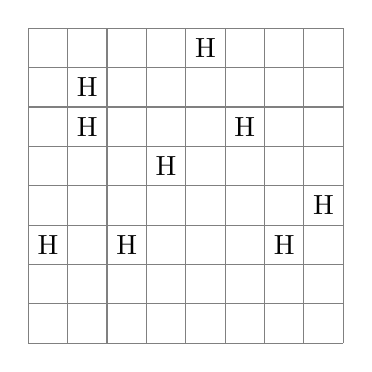
\begin{tikzpicture}

\draw[step=0.5cm,color=gray] (-1,-1) grid (3,3);
\node at (1.25,+2.75) {H};
\node at (-.25,+2.25) {H};
\node at (-0.25,+1.75) {H};
\node at (+0.75,+1.25) {H};
\node at (1.75,+1.75) {H};
\node at (2.75,+0.75) {H};
\node at (+2.25,0.25) {H};
\node at (+.25,+0.25) {H};
\node at (-.75,.25) {H};
\end{tikzpicture}
\end{minipage}
}





\hfill \break
\break
Where as the Shortest path method still gives the optimal number of paths which is 3. This does not mean that our  \textbf{Shortest} Algorithm is correct only that it is better then our \textbf{Most Houses} Algorithm.
\hfill \break
\break
\\
\newpage
\hfill \break
\break
AH = Array of tuple coordinates of Houses pre-sorted by y values
\newline
numberOfHouse = len(AH)
\newline
routes =  2D matrix with Mailmen as the first level and their routes as tuples as the inner array as tuples
\newline
currentRow = 0
\newline
currentCol = 0
\newline
numberOfMailMen = 0
\newline
N =  max number of rows and col in NxN matrix
\begin{lstlisting}
while(len(numberOfHouse) > 0)
    while (currentCol < N or currentRow < N):
            colIndex = (0,0)
            rowIndex = (0,0)
            for index to len(AH) :
                   if AH[index].0 == currentRow and rowIndex == (0,0):
                        rowIndex = AH[index]
                        continue
                   if AH[index].1 == currentCol and colIndex == (0,0) :
                        colIndex = AH[index]
                        continue
            deltaX =  rowIndex.0 - currentRow
            deltaY = colIndex.1 - currentCol
            if deltaX > deltaY:
                go down
                currentCol++
                routes[numberOfMailMen] = (currentRow,currentCol)
            if  deltaX < deltaY
                go right
                currentRow++
                routes[numberOfMailMen] = (currentRow,currentCol)
            for index to len(AH):
                if AH[index].0 == currentRow & AH[index].1 == currentCol:
                    numberOfHouse = numberOfHouse - 1
            if currentRow == (N-1) and currentRow == (N-1):
                numberOfMailMen = numberOfMailMen + 1
                currentCol = 0
                currentRow = 0
                
            



        
        
           
            
            
                
                
    
\end{lstlisting}
\\
\\
\newpage
\hfill \break
\break
Not looking at the code above we will now look at the problem to try find its complexity in a more general sense.
We are trying to find a algorithm that runs in poly-time, to do this we would like to show that in the worst case we are within the bounds of a poly-time complexity. 
\\
\\
\\
With this is mind let us look at the worst case where houses are on a reverse diagonal from our starting position.
\hfill \break
\break
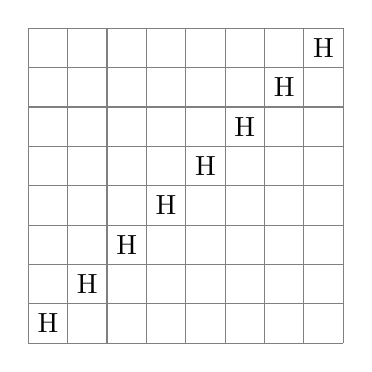
\begin{tikzpicture}

\draw[step=0.5cm,color=gray] (-1,-1) grid (3,3);
\node at (2.75,+2.75) {H};
\node at (2.25,+2.25) {H};
\node at (1.75,+1.75) {H};
\node at (.75,+0.75) {H};
\node at (+1.25,+1.25) {H};
\node at (-.75,-.75) {H};
\node at (+.25,+0.25) {H};
\node at (-.25,-.25) {H};
\end{tikzpicture}
\hfill \break
\break
The above Grid showcases the worst case input for our algorithm. Where there is 8 house on the inverse diagonal from our starting positions (0,0). In this example we can clearly see that due to our Mailmens ability to only move down and to the right we will need at least N number of Mailmen to visit all of our houses. 
\hfill \break
\break
So in our worst case we need \textit{n} Mailmen for \textit{n} houses, in other words the number of Mailmen equals \textit{n}. Now each Mailman moves 2\textit{n}-1 spaces on his route. So this means that if we have the worst case input where the houses are on an inverse angle from our start position, we will need \textit{n} Mailmen who each move 2\textit{n}-1 times.
This gives us a complexity of \textit{n}(2\textit{n}-1), leading to a 2\textit{$n^2$} - \textit{n} which is in \textit{O($n^2$)}.

\hfill \break
\break
Now that we have the worst case run-time of an algorithm not including data structures or anything we need to keep track of let us look at the run-time of the algorithm above.

 


\pagebreak
\part{Marking Graphs}
Question 2.1
\\
\\
For this question my Graph is not the minimal number of Nodes needed to create a counter example. However I believe that the Graph i have given helps to illustrate a key insight into creating a counter example that haws the potential to give you an Optimal Solution. The key to breaking this Algorithm comes when a tie occurs. When there are multiple max degree Nodes the Algorithm will have to choice which one to \textbf{mark}. In the example below we have 9 Nodes with Degree 3 which also happens to be the maximum degree. This creates our Tie condition and since we solve a Tie by \enquote{\textbf{pick[ing] any one vertices of maximal degree}}, if this Algorithm is optimal it shouldn't matter which one we pick.
\\
\\
However in this graph I have \enquote{Insulated} the nine nodes in a particular way that if the wrong Node is selected in a particular order the outermost Nodes become isolated and will need to be marked individually.  
\hfill \break
\break
\textbf{Non-optimal choice}
\begin{steps}
  \item \textbf{Step 1:} Start at Node 3 and \textbf{mark} it
  \item \textbf{Step 2:} Remove Node 3, 2, 12 and 6 because they are now next to a \textbf{marked} Node
  \item \textbf{Step 3:} Now we have a Choice between 4, 5, 7, 11, 8 lets pick 5 and \textbf{marked} it
  \item \textbf{Step 4:} Remove Nodes 4 and 5 because they are now next to a \textbf{marked} Node
  \item \textbf{Step 5:} Now we are left with Node 8 with the Highest Degree so we \textbf{mark} it
  \item \textbf{Step 6:} Remove Nodes 8, 10 and 11 because they are now next to a \textbf{marked} Node
  \item \textbf{Step 7:} Now remaining Nodes 1 and 9 will need to be \textbf{marked} individually 

\end{steps}
\hfill \break

\begin{center}
\newpage
 Step 1 \textbf{Non-optimal}
 \hfill \break
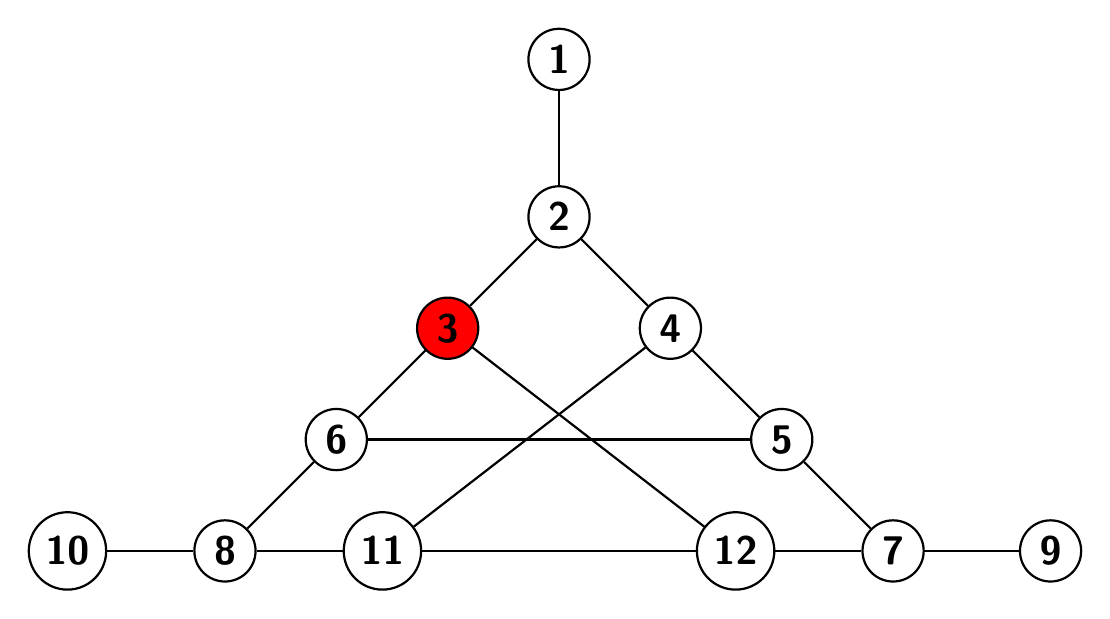
\begin{tikzpicture}[auto, node distance=2cm, every loop/.style={},
                    thick,main node/.style={circle,draw,font=\sffamily\Large\bfseries}]

  \node[main node] (1) {1};
  \node[main node] (2) [below of=1] {2};
  \node[main node,fill=red] (3) [below  left of=2] {3};
  \node[main node] (4) [below  right of=2] {4};
  \node[main node] (5) [below  right of=4] {5};
  \node[main node] (6) [below  left of=3] {6};
  \node[main node] (7) [below  right of=5] {7};
  \node[main node] (8) [below  left of=6] {8};
  \node[main node] (9) [  right of=7] {9};
  \node[main node] (10) [  left of=8] {10};
  \node[main node] (11) [  right of=8] {11};
  \node[main node] (12) [  left of=7] {12};
         
         
\path[every node/.style={font=\sffamily\small}]
    (1) edge node [left] {} (2)
    (2) edge node [right] {} (4)
    (2) edge node [right] {} (3)
    (3) edge node [right] {} (6)
    (6) edge node [right] {} (8)
    (4) edge node [right] {} (5)
     (5) edge node [right] {} (7)
      (7) edge node [right] {} (9)
       (10) edge node [right] {} (8)
        (8) edge node [right] {} (11)
         (11) edge node [right] {} (12)
          (12) edge node [right] {} (7)
          (3) edge node [right] {} (12)
          (4) edge node [right] {} (11)
          (6) edge node [right] {} (5);
    

\end{tikzpicture}
 \hfill \break
 Step 2 \textbf{Non-optimal}
 \hfill \break
\begin{tikzpicture}[auto, node distance=2cm, every loop/.style={},
                    thick,main node/.style={circle,draw,font=\sffamily\Large\bfseries}]

  \node[main node] (1) {1};
  \node[main node,draw=none] (2) [below of=1] {};
  \node[main node,draw=none] (3) [below  left of=2] {};
  \node[main node] (4) [below  right of=2] {4};
  \node[main node] (5) [below  right of=4] {5};
  \node[main node,draw=none] (6) [below  left of=3] {};
  \node[main node] (7) [below  right of=5] {7};
  \node[main node] (8) [below  left of=6] {8};
  \node[main node] (9) [  right of=7] {9};
  \node[main node] (10) [  left of=8] {10};
  \node[main node] (11) [  right of=8] {11};
  \node[main node,draw=none] (12) [  left of=7] {};
         
         
\path[every node/.style={font=\sffamily\small}]
   
   

 
 
    (4) edge node [right] {} (5)
     (5) edge node [right] {} (7)
      (7) edge node [right] {} (9)
       (10) edge node [right] {} (8)
        (8) edge node [right] {} (11)
         
      
          (4) edge node [right] {} (11)
  ;
    

\end{tikzpicture}
\newpage
 \hfill \break
 Step 3 \textbf{Non-optimal}
 \hfill \break
\begin{tikzpicture}[auto, node distance=2cm, every loop/.style={},
                    thick,main node/.style={circle,draw,font=\sffamily\Large\bfseries}]

  \node[main node] (1) {1};
  \node[main node,draw=none] (2) [below of=1] {};
  \node[main node,draw=none] (3) [below  left of=2] {};
  \node[main node] (4) [below  right of=2] {4};
  \node[main node,fill=red] (5) [below  right of=4] {5};
  \node[main node,draw=none] (6) [below  left of=3] {};
  \node[main node] (7) [below  right of=5] {7};
  \node[main node] (8) [below  left of=6] {8};
  \node[main node] (9) [  right of=7] {9};
  \node[main node] (10) [  left of=8] {10};
  \node[main node] (11) [  right of=8] {11};
  \node[main node,draw=none] (12) [  left of=7] {};
         
         
\path[every node/.style={font=\sffamily\small}]
   
   

 
 
    (4) edge node [right] {} (5)
     (5) edge node [right] {} (7)
      (7) edge node [right] {} (9)
       (10) edge node [right] {} (8)
        (8) edge node [right] {} (11)
         
      
          (4) edge node [right] {} (11)
  ;
    

\end{tikzpicture}
 \hfill \break
 Step 4 \textbf{Non-optimal}
 \hfill \break
\begin{tikzpicture}[auto, node distance=2cm, every loop/.style={},
                    thick,main node/.style={circle,draw,font=\sffamily\Large\bfseries}]

  \node[main node] (1) {1};
  \node[main node,draw=none] (2) [below of=1] {};
  \node[main node,draw=none] (3) [below  left of=2] {};
  \node[main node,draw=none] (4) [below  right of=2] {};
  \node[main node,draw=none] (5) [below  right of=4] {};
  \node[main node,draw=none] (6) [below  left of=3] {};
  \node[main node,draw=none] (7) [below  right of=5] {};
  \node[main node] (8) [below  left of=6] {8};
  \node[main node] (9) [  right of=7] {9};
  \node[main node] (10) [  left of=8] {10};
  \node[main node] (11) [  right of=8] {11};
  \node[main node,draw=none] (12) [  left of=7] {};
         
         
\path[every node/.style={font=\sffamily\small}]
   
  
   
       (10) edge node [right] {} (8)
        (8) edge node [right] {} (11)
         
    
  ;
    

\end{tikzpicture}
\newpage
 \hfill \break
 Step 5 \textbf{Non-optimal}
 \hfill \break
\begin{tikzpicture}[auto, node distance=2cm, every loop/.style={},
                    thick,main node/.style={circle,draw,font=\sffamily\Large\bfseries}]

  \node[main node] (1) {1};
  \node[main node,draw=none] (2) [below of=1] {};
  \node[main node,draw=none] (3) [below  left of=2] {};
  \node[main node,draw=none] (4) [below  right of=2] {};
  \node[main node,draw=none] (5) [below  right of=4] {};
  \node[main node,draw=none] (6) [below  left of=3] {};
  \node[main node,draw=none] (7) [below  right of=5] {};
  \node[main node,fill=red] (8) [below  left of=6] {8};
  \node[main node] (9) [  right of=7] {9};
  \node[main node] (10) [  left of=8] {10};
  \node[main node] (11) [  right of=8] {11};
  \node[main node,draw=none] (12) [  left of=7] {};
         
         
\path[every node/.style={font=\sffamily\small}]
   
  
   
       (10) edge node [right] {} (8)
        (8) edge node [right] {} (11)
         
    
  ;
    

\end{tikzpicture}
 \hfill \break
 Step 6 \textbf{Non-optimal}
 \hfill \break \break
\begin{tikzpicture}[auto, node distance=2cm, every loop/.style={},
                    thick,main node/.style={circle,draw,font=\sffamily\Large\bfseries}]

  \node[main node] (1) {1};
  \node[main node,draw=none] (2) [below of=1] {};
  \node[main node,draw=none] (3) [below  left of=2] {};
  \node[main node,draw=none] (4) [below  right of=2] {};
  \node[main node,draw=none] (5) [below  right of=4] {};
  \node[main node,draw=none] (6) [below  left of=3] {};
  \node[main node,draw=none] (7) [below  right of=5] {};
  \node[main node,draw=none] (8) [below  left of=6] {};
  \node[main node] (9) [  right of=7] {9};
  \node[main node,draw=none] (10) [  left of=8] {};
  \node[main node,draw=none] (11) [  right of=8] {};
  \node[main node,draw=none] (12) [  left of=7] {};
         
    

\end{tikzpicture}
\newpage
 \hfill \break
 Step 7 \textbf{Non-optimal}
 \hfill \break
 \break
 
\begin{tikzpicture}[auto, node distance=2cm, every loop/.style={},
                    thick,main node/.style={circle,draw,font=\sffamily\Large\bfseries}]

  \node[main node,fill=red] (1) {1};
  \node[main node,draw=none] (2) [below of=1] {};
  \node[main node,draw=none] (3) [below  left of=2] {};
  \node[main node,draw=none] (4) [below  right of=2] {};
  \node[main node,draw=none] (5) [below  right of=4] {};
  \node[main node,draw=none] (6) [below  left of=3] {};
  \node[main node,draw=none] (7) [below  right of=5] {};
  \node[main node,draw=none] (8) [below  left of=6] {};
  \node[main node,fill=red] (9) [  right of=7] {9};
  \node[main node,draw=none] (10) [  left of=8] {};
  \node[main node,draw=none] (11) [  right of=8] {};
  \node[main node,draw=none] (12) [  left of=7] {};
         
    

\end{tikzpicture}
\end{center}
\hfill \break
This leads to five marked Nodes
\hfill \break

\hfill \break
\break
\textbf{Optimal choice}
\begin{steps}
  \item \textbf{Step 1:} Start at Node 2 and \textbf{mark} it
  \item \textbf{Step 2:} Remove Node 2, 1, 3 and 4 because they are now next to a \textbf{marked} Node
  \item \textbf{Step 3:} Next choose Node 8 and \textbf{mark} it
  \item \textbf{Step 4:} Remove Nodes 8, 10, 6 and 11 because they are now next to a \textbf{marked} Node
  \item \textbf{Step 5:} Next choose Node 7 and \textbf{mark} it
  \item \textbf{Step 6:} Remove Nodes 7, 5, 12 and 9 because they are now next to a \textbf{marked} Node

\end{steps}
\hfill \break

\begin{center}
\newpage
 Step 1 \textbf{Optimal}
 \hfill \break
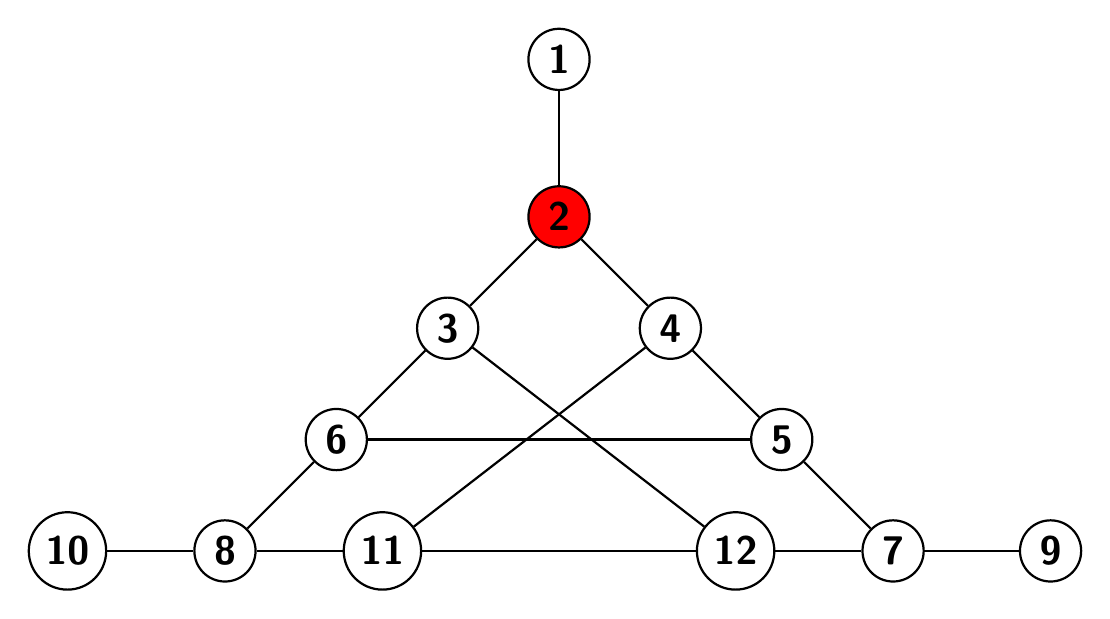
\begin{tikzpicture}[auto, node distance=2cm, every loop/.style={},
                    thick,main node/.style={circle,draw,font=\sffamily\Large\bfseries}]

  \node[main node] (1) {1};
  \node[main node,fill=red] (2) [below of=1] {2};
  \node[main node] (3) [below  left of=2] {3};
  \node[main node] (4) [below  right of=2] {4};
  \node[main node] (5) [below  right of=4] {5};
  \node[main node] (6) [below  left of=3] {6};
  \node[main node] (7) [below  right of=5] {7};
  \node[main node] (8) [below  left of=6] {8};
  \node[main node] (9) [  right of=7] {9};
  \node[main node] (10) [  left of=8] {10};
  \node[main node] (11) [  right of=8] {11};
  \node[main node] (12) [  left of=7] {12};
         
         
\path[every node/.style={font=\sffamily\small}]
    (1) edge node [left] {} (2)
    (2) edge node [right] {} (4)
    (2) edge node [right] {} (3)
    (3) edge node [right] {} (6)
    (6) edge node [right] {} (8)
    (4) edge node [right] {} (5)
     (5) edge node [right] {} (7)
      (7) edge node [right] {} (9)
       (10) edge node [right] {} (8)
        (8) edge node [right] {} (11)
         (11) edge node [right] {} (12)
          (12) edge node [right] {} (7)
          (3) edge node [right] {} (12)
          (4) edge node [right] {} (11)
          (6) edge node [right] {} (5);
    

\end{tikzpicture}
 Step 2 \textbf{Optimal}
 \hfill \break
\begin{tikzpicture}[auto, node distance=2cm, every loop/.style={},
                    thick,main node/.style={circle,draw,font=\sffamily\Large\bfseries}]

  \node[main node,draw=none] (1) {};
  \node[main node,draw=none] (2) [below of=1] {};
  \node[main node,draw=none] (3) [below  left of=2] {};
  \node[main node,draw=none] (4) [below  right of=2] {};
  \node[main node] (5) [below  right of=4] {5};
  \node[main node] (6) [below  left of=3] {6};
  \node[main node] (7) [below  right of=5] {7};
  \node[main node] (8) [below  left of=6] {8};
  \node[main node] (9) [  right of=7] {9};
  \node[main node] (10) [  left of=8] {10};
  \node[main node] (11) [  right of=8] {11};
  \node[main node] (12) [  left of=7] {12};
         
         
\path[every node/.style={font=\sffamily\small}]

  
  
  
    (6) edge node [right] {} (8)

     (5) edge node [right] {} (7)
      (7) edge node [right] {} (9)
       (10) edge node [right] {} (8)
        (8) edge node [right] {} (11)
         (11) edge node [right] {} (12)
          (12) edge node [right] {} (7)
         
         
          (6) edge node [right] {} (5);
    

\end{tikzpicture}
\newpage
Step 3 \textbf{Optimal}
 \hfill \break
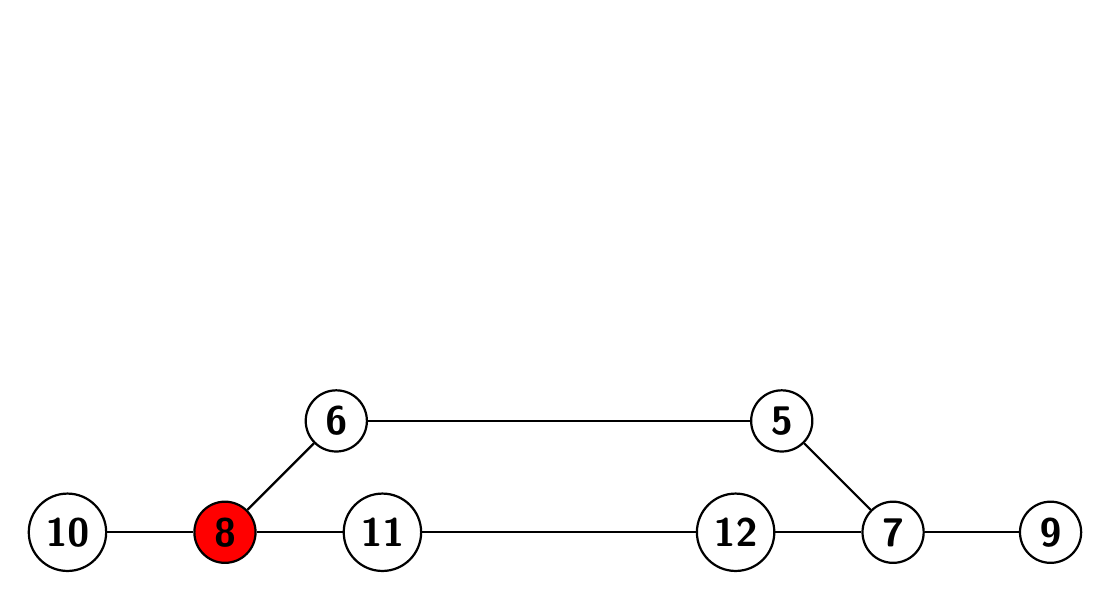
\begin{tikzpicture}[auto, node distance=2cm, every loop/.style={},
                    thick,main node/.style={circle,draw,font=\sffamily\Large\bfseries}]

  \node[main node,draw=none] (1) {};
  \node[main node,draw=none] (2) [below of=1] {};
  \node[main node,draw=none] (3) [below  left of=2] {};
  \node[main node,draw=none] (4) [below  right of=2] {};
  \node[main node] (5) [below  right of=4] {5};
  \node[main node] (6) [below  left of=3] {6};
  \node[main node] (7) [below  right of=5] {7};
  \node[main node,fill=red] (8) [below  left of=6] {8};
  \node[main node] (9) [  right of=7] {9};
  \node[main node] (10) [  left of=8] {10};
  \node[main node] (11) [  right of=8] {11};
  \node[main node] (12) [  left of=7] {12};
         
         
\path[every node/.style={font=\sffamily\small}]

  
  
  
    (6) edge node [right] {} (8)

     (5) edge node [right] {} (7)
      (7) edge node [right] {} (9)
       (10) edge node [right] {} (8)
        (8) edge node [right] {} (11)
         (11) edge node [right] {} (12)
          (12) edge node [right] {} (7)
         
         
          (6) edge node [right] {} (5);
    

\end{tikzpicture}
Step 4 \textbf{Optimal}
 \hfill \break
\begin{tikzpicture}[auto, node distance=2cm, every loop/.style={},
                    thick,main node/.style={circle,draw,font=\sffamily\Large\bfseries}]

  \node[main node,draw=none] (1) {};
  \node[main node,draw=none] (2) [below of=1] {};
  \node[main node,draw=none] (3) [below  left of=2] {};
  \node[main node,draw=none] (4) [below  right of=2] {};
  \node[main node] (5) [below  right of=4] {5};
  \node[main node,draw=none] (6) [below  left of=3] {};
  \node[main node] (7) [below  right of=5] {7};
  \node[main node,draw=none] (8) [below  left of=6] {};
  \node[main node] (9) [  right of=7] {9};
  \node[main node,draw=none] (10) [  left of=8] {};
  \node[main node,draw=none] (11) [  right of=8] {};
  \node[main node] (12) [  left of=7] {12};
         
         
\path[every node/.style={font=\sffamily\small}]

  
  
  
   

     (5) edge node [right] {} (7)
      (7) edge node [right] {} (9)
       
      
      
          (12) edge node [right] {} (7)
   ;
    

\end{tikzpicture}
\newpage
Step 5 \textbf{Optimal}
 \hfill \break
\begin{tikzpicture}[auto, node distance=2cm, every loop/.style={},
                    thick,main node/.style={circle,draw,font=\sffamily\Large\bfseries}]

  \node[main node,draw=none] (1) {};
  \node[main node,draw=none] (2) [below of=1] {};
  \node[main node,draw=none] (3) [below  left of=2] {};
  \node[main node,draw=none] (4) [below  right of=2] {};
  \node[main node] (5) [below  right of=4] {5};
  \node[main node,draw=none] (6) [below  left of=3] {};
  \node[main node,fill=red] (7) [below  right of=5] {7};
  \node[main node,draw=none] (8) [below  left of=6] {};
  \node[main node] (9) [  right of=7] {9};
  \node[main node,draw=none] (10) [  left of=8] {};
  \node[main node,draw=none] (11) [  right of=8] {};
  \node[main node] (12) [  left of=7] {12};
         
         
\path[every node/.style={font=\sffamily\small}]

  
  
  
   

     (5) edge node [right] {} (7)
      (7) edge node [right] {} (9)
       
      
      
          (12) edge node [right] {} (7)
   ;
    

\end{tikzpicture}

\end{center}
\hfill \break
This leads to an Optimal number of marked Nodes which is 3
\hfill \break






\pagebreak
\hfill \break
\break
Question 2.2
\\
\\
The Graph I have given below is not the smallest number of nodes that you can use to give a counter example. In fact key to the counter example comes by denying the Algorithm an even edge and forcing it to pick an odd edge that is not going to give the Optimal Solution. The flaw with this algorithm like the one above comes from when there is a tie. particularly when there is no even Node to choose from and there by  \\\enquote{\textbf{mark[ing] any one vertex of odd degree}}.
\hfill \break
\break
\textbf{Non-optimal choice}
\begin{steps}
  \item \textbf{Step 1:} Start at Node 2 and \textbf{mark} it
  \item \textbf{Step 2:} Remove Node 2, 3 and 1 because they are now next to a \textbf{marked} Node
  \item \textbf{Step 3:} There are no Even Nodes so pick any Odd Node in this case\\ Node 4 and \textbf{mark} it
  \item \textbf{Step 4:} Remove Nodes 4 and 5 because they are now next to a \textbf{marked} Node
  \item \textbf{Step 5:} Now remaining Nodes 7 and 6 will need to be \textbf{marked} individually 
\end{steps}
\hfill \break




\noindent\fboxsep{%
\begin{minipage}{14em}
 \centering
 Step 1 \textbf{non-optimal}
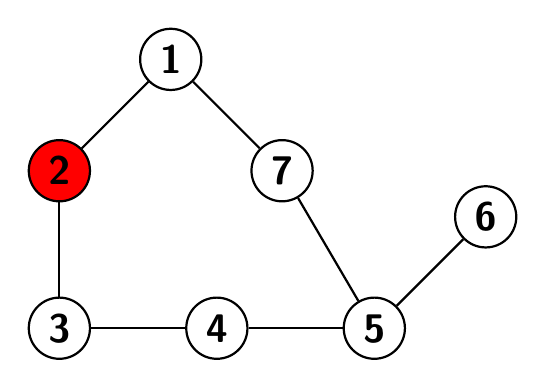
\begin{tikzpicture}[auto, node distance=2cm, every loop/.style={},
                    thick,main node/.style={circle,draw,font=\sffamily\Large\bfseries}]

  \node[main node] (1) {1};
  \node[main node,fill=red] (2) [below left of=1] {2};
\node[main node] (3) [below  of=2] {3};
\node[main node] (4) [right  of=3] {4};
\node[main node] (5) [ right  of=4] {5};
\node[main node] (6) [above right  of=5] {6};
\node[main node] (7) [below right  of=1] {7};


\path[every node/.style={font=\sffamily\small}]
    (1) edge node [left] {} (2)
    (2) edge node [left] {} (3)
    (3) edge node [left] {} (4)
    (4) edge node [left] {} (5)
    (5) edge node [left] {} (6)
    (5) edge node [left] {} (7)
    (7) edge node [left] {} (1);
 
\end{tikzpicture}
\end{minipage}}%
\hfill%
\fboxsep{%
\begin{minipage}{14em}
 \centering
 Step 2 \textbf{non-optimal}
\begin{tikzpicture}[auto, node distance=2cm, every loop/.style={},
                    thick,main node/.style={circle,draw,font=\sffamily\Large\bfseries}]
  \node[main node,draw=none] (1) {};
  \node[main node,draw=none] (2) [below left of=1] {};
\node[main node,draw=none] (3) [below  of=2] {};
\node[main node] (4) [right  of=3] {4};
\node[main node] (5) [ right  of=4] {5};
\node[main node] (6) [above right  of=5] {6};
\node[main node] (7) [below right  of=1] {7};


\path[every node/.style={font=\sffamily\small}]
  
   
   
    (4) edge node [left] {} (5)
    (5) edge node [left] {} (6)
    (5) edge node [left] {} (7)
  
 
\end{tikzpicture}
\end{minipage}
}
\hfill \break
\break


\noindent\fboxsep{%
\begin{minipage}{14em}
 \centering
 Step 3 \textbf{non-optimal}
\begin{tikzpicture}[auto, node distance=2cm, every loop/.style={},
                    thick,main node/.style={circle,draw,font=\sffamily\Large\bfseries}]

  \node[main node,draw=none] (1) {};
  \node[main node,draw=none] (2) [below left of=1] {};
\node[main node,draw=none] (3) [below  of=2] {};
\node[main node,fill=red] (4) [right  of=3] {4};
\node[main node] (5) [ right  of=4] {5};
\node[main node] (6) [above right  of=5] {6};
\node[main node] (7) [below right  of=1] {7};


\path[every node/.style={font=\sffamily\small}]
  
   
   
    (4) edge node [left] {} (5)
    (5) edge node [left] {} (6)
    (5) edge node [left] {} (7)
   
 
\end{tikzpicture}
\end{minipage}}%
\hfill%
\fboxsep{%
\begin{minipage}{14em}
 \centering
 Step 4 \textbf{non-optimal}
\begin{tikzpicture}[auto, node distance=2cm, every loop/.style={},
                    thick,main node/.style={circle,draw,font=\sffamily\Large\bfseries}]
   \node[main node,draw=none] (1) {};
  \node[main node,draw=none] (2) [below left of=1] {};
\node[main node,draw=none] (3) [below  of=2] {};
\node[main node,draw=none] (4) [right  of=3] {};
\node[main node,draw=none] (5) [ right  of=4] {};
\node[main node] (6) [above right  of=5] {6};
\node[main node] (7) [below right  of=1] {7};


\path[every node/.style={font=\sffamily\small}]
  
   
   
 
   
 
\end{tikzpicture}
\end{minipage}
}

\begin{center}
\newpage
 Step 5 \textbf{non-optimal}
 
\begin{tikzpicture}[auto, node distance=2cm, every loop/.style={},
                    thick,main node/.style={circle,draw,font=\sffamily\Large\bfseries}]
   \node[main node,draw=none] (1) {};
  \node[main node,draw=none] (2) [below left of=1] {};
\node[main node,draw=none] (3) [below  of=2] {};
\node[main node,draw=none] (4) [right  of=3] {};
\node[main node,draw=none] (5) [ right  of=4] {};
\node[main node,fill=red] (6) [above right  of=5] {6};
\node[main node,fill=red] (7) [below right  of=1] {7};


\path[every node/.style={font=\sffamily\small}]
  
   
   
 
   
 
\end{tikzpicture}
\hfill \break
This leads to four \textbf{Marked} Nodes
\hfill \break

\end{center}
\newpage
\hfill \break
\break
\textbf{Optimal choice}
\begin{steps}
  \item \textbf{Step 1:} Start at Node 2 and \textbf{mark} it
  \item \textbf{Step 2:} Remove Node 2, 3 and 1 because they are now next to a \textbf{marked} Node
  \item \textbf{Step 3:} Now \textbf{mark} 5
  \item \textbf{Step 4:} Remove Nodes 5, 4,7 and 6 because they are now next to a \textbf{marked} Node
\end{steps}
\hfill \break
\break

\noindent\fboxsep{%
\begin{minipage}{14em}
 \centering
 Step 1 \textbf{Optimal}
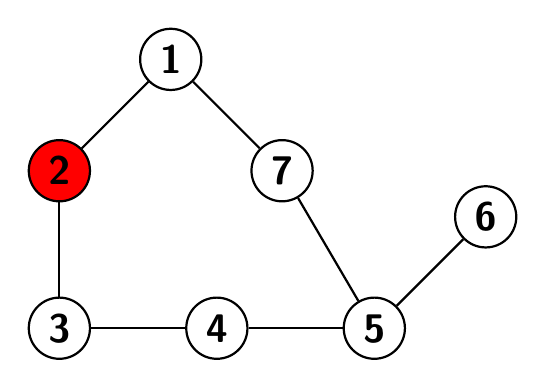
\begin{tikzpicture}[auto, node distance=2cm, every loop/.style={},
                    thick,main node/.style={circle,draw,font=\sffamily\Large\bfseries}]

  \node[main node] (1) {1};
  \node[main node,fill=red] (2) [below left of=1] {2};
\node[main node] (3) [below  of=2] {3};
\node[main node] (4) [right  of=3] {4};
\node[main node] (5) [ right  of=4] {5};
\node[main node] (6) [above right  of=5] {6};
\node[main node] (7) [below right  of=1] {7};


\path[every node/.style={font=\sffamily\small}]
    (1) edge node [left] {} (2)
    (2) edge node [left] {} (3)
    (3) edge node [left] {} (4)
    (4) edge node [left] {} (5)
    (5) edge node [left] {} (6)
    (5) edge node [left] {} (7)
    (7) edge node [left] {} (1);
 
\end{tikzpicture}
\end{minipage}}%
\hfill%
\fboxsep{%
\begin{minipage}{14em}
 \centering
 Step 2 \textbf{Optimal}
\begin{tikzpicture}[auto, node distance=2cm, every loop/.style={},
                    thick,main node/.style={circle,draw,font=\sffamily\Large\bfseries}]
  \node[main node,draw=none] (1) {};
  \node[main node,draw=none] (2) [below left of=1] {};
\node[main node,draw=none] (3) [below  of=2] {};
\node[main node] (4) [right  of=3] {4};
\node[main node] (5) [ right  of=4] {5};
\node[main node] (6) [above right  of=5] {6};
\node[main node] (7) [below right  of=1] {7};


\path[every node/.style={font=\sffamily\small}]
  
   
   
    (4) edge node [left] {} (5)
    (5) edge node [left] {} (6)
    (5) edge node [left] {} (7)
  
 
\end{tikzpicture}
\end{minipage}
}
\hfill \break
\break


\noindent\fboxsep{%
\begin{minipage}{14em}
 \centering
 Step 3 \textbf{Optimal}
\begin{tikzpicture}[auto, node distance=2cm, every loop/.style={},
                    thick,main node/.style={circle,draw,font=\sffamily\Large\bfseries}]

  \node[main node,draw=none] (1) {};
  \node[main node,draw=none] (2) [below left of=1] {};
\node[main node,draw=none] (3) [below  of=2] {};
\node[main node] (4) [right  of=3] {4};
\node[main node,fill=red] (5) [ right  of=4] {5};
\node[main node] (6) [above right  of=5] {6};
\node[main node] (7) [below right  of=1] {7};


\path[every node/.style={font=\sffamily\small}]
  
   
   
    (4) edge node [left] {} (5)
    (5) edge node [left] {} (6)
    (5) edge node [left] {} (7)
   
 
\end{tikzpicture}
\end{minipage}}%
\hfill%
\fboxsep{%
\begin{minipage}{14em}
 \centering
 Step 4 \textbf{Optimal}
\begin{tikzpicture}[auto, node distance=2cm, every loop/.style={},
                    thick,main node/.style={circle,draw,font=\sffamily\Large\bfseries}]
   \node[main node,draw=none] (1) {};
  \node[main node,draw=none] (2) [below left of=1] {};
\node[main node,draw=none] (3) [below  of=2] {};
\node[main node,draw=none] (4) [right  of=3] {};
\node[main node,draw=none] (5) [ right  of=4] {};
\node[main node,draw=none] (6) [above right  of=5] {};
\node[main node,draw=none] (7) [below right  of=1] {};


\path[every node/.style={font=\sffamily\small}]
  
   
   
 
   
 
\end{tikzpicture}
\end{minipage}
}
\hfill \break
\break

This leads to two \textbf{Marked} Nodes
\hfill \break
\break























\pagebreak
\hfill \break
\break
Question 2.3
\hfill \break
\break
This question was by far the more difficult of all three. How I decided to tackle the problem was to control the entry points by which the Algorithm could enter the graph. So I created a graph with only two entry points both with the least degree. One of the entry points would give the optimal solution while the other would give the a satisfactory solution but not optimal.
\hfill \break
\break
\textbf{Non-optimal choice}
\begin{steps}
  \item \textbf{Step 1:} Start at Node 1
  \item \textbf{Step 2:} Move to Node 2 because it has a Degree of 3 and \textbf{mark} it
  \item \textbf{Step 3:} Remove Node 1, 5 and 3 because they are now next to a \textbf{marked} Node
  \item \textbf{Step 4:} Only Nodes left are 6 and 4 which are not connected by and edge so they each must be marked themselves
\end{steps}
\hfill \break
\break
This leads to three marked Nodes
\begin{center}

\end{center}
\noindent\fboxsep{%
\begin{minipage}{14em}
 \centering
 Step 1 \textbf{non-optimal}
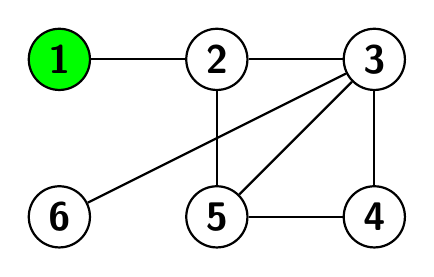
\begin{tikzpicture}[auto, node distance=2cm, every loop/.style={},
                    thick,main node/.style={circle,draw,font=\sffamily\Large\bfseries}]

  \node[main node,fill=green] (1) {1};
  \node[main node] (2) [ right of=1] {2};
    \node[main node] (3) [ right of=2] {3};
      \node[main node] (4) [ below of=3] {4};
        \node[main node] (5) [ left of=4] {5};
          \node[main node] (6) [ left of=5] {6};

\path[every node/.style={font=\sffamily\small}]
    (1) edge node [left] {} (2)
    (2) edge node [left] {} (3)
    (3) edge node [left] {} (4)
    (4) edge node [left] {} (5)
   
    (3) edge node [left] {} (5)
    (6) edge node [left] {} (3)
    (2) edge node [left] {} (5);
 
\end{tikzpicture}
\end{minipage}}%
\hfill%
\fboxsep{%
\begin{minipage}{14em}
 \centering
 Step 2 \textbf{non-optimal}
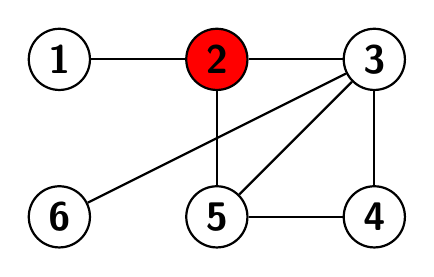
\begin{tikzpicture}[auto, node distance=2cm, every loop/.style={},
                    thick,main node/.style={circle,draw,font=\sffamily\Large\bfseries}]

  \node[main node] (1) {1};
  \node[main node,fill=red] (2) [ right of=1] {2};
    \node[main node] (3) [ right of=2] {3};
      \node[main node] (4) [ below of=3] {4};
        \node[main node] (5) [ left of=4] {5};
          \node[main node] (6) [ left of=5] {6};

\path[every node/.style={font=\sffamily\small}]
    (1) edge node [left] {} (2)
    (2) edge node [left] {} (3)
    (3) edge node [left] {} (4)
    (4) edge node [left] {} (5)
   
    (3) edge node [left] {} (5)
    (6) edge node [left] {} (3)
    (2) edge node [left] {} (5);
 
\end{tikzpicture}
\end{minipage}
}
\\
\\
\\
\noindent\fboxsep{%
\begin{minipage}{14em}
 \centering
 
 Step 3 \textbf{non-optimal}
\begin{tikzpicture}[auto, node distance=2cm, every loop/.style={},
                    thick,main node/.style={circle,draw,font=\sffamily\Large\bfseries}]

  \node[main node,draw=none] (1) {};
  \node[main node,draw=none] (2) [ right of=1] {};
    \node[main node,draw=none] (3) [ right of=2] {};
      \node[main node] (4) [ below of=3] {4};
        \node[main node,draw=none] (5) [ left of=4] {};
          \node[main node] (6) [ left of=5] {6};


    
    
   
    
  

 
\end{tikzpicture}
\end{minipage}}%
\hfill%
\fboxsep{%
\begin{minipage}{14em}
 \centering
 Step 4 \textbf{non-optimal}
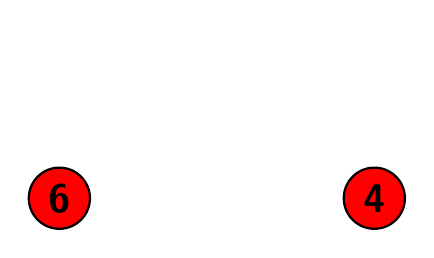
\begin{tikzpicture}[auto, node distance=2cm, every loop/.style={},
                    thick,main node/.style={circle,draw,font=\sffamily\Large\bfseries}]

\node[main node,draw=none] (1) {};
  \node[main node,draw=none] (2) [ right of=1] {};
    \node[main node,draw=none] (3) [ right of=2] {};
      \node[main node,fill=red] (4) [ below of=3] {4};
        \node[main node,draw=none] (5) [ left of=4] {};
          \node[main node,fill=red] (6) [ left of=5] {6};
 
\end{tikzpicture}
\end{minipage}
}

\pagebreak
\hfill \break
\break
\textbf{Optimal choice}
\begin{steps}
  \item \textbf{Step 1:} Start at Node 6
  \item \textbf{Step 2:} Move to Node 3 because it has a Degree of 4 and \textbf{mark} it
  \item \textbf{Step 3:} Remove Node 3, 5, 2 and 4 because they are now next to a \textbf{marked} Node
  \item \textbf{Step 4:} Only Node left is 1 and must be \textbf{marked} itself
\end{steps}
\hfill \break
\break
This leads to only two marked Nodes being needed and is the Optimal Solution for this Graph

\begin{center}

\end{center}
\noindent\fboxsep{%
\begin{minipage}{14em}
 \centering
 Step 1 \textbf{Optimal}
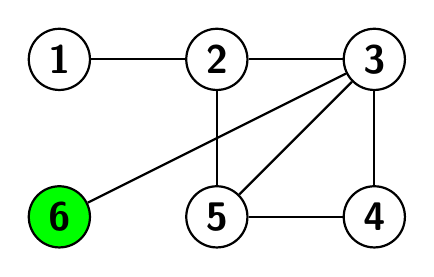
\begin{tikzpicture}[auto, node distance=2cm, every loop/.style={},
                    thick,main node/.style={circle,draw,font=\sffamily\Large\bfseries}]

  \node[main node] (1) {1};
  \node[main node] (2) [ right of=1] {2};
    \node[main node] (3) [ right of=2] {3};
      \node[main node] (4) [ below of=3] {4};
        \node[main node] (5) [ left of=4] {5};
          \node[main node,fill=green] (6) [ left of=5] {6};

\path[every node/.style={font=\sffamily\small}]
    (1) edge node [left] {} (2)
    (2) edge node [left] {} (3)
    (3) edge node [left] {} (4)
    (4) edge node [left] {} (5)
   
    (3) edge node [left] {} (5)
    (6) edge node [left] {} (3)
    (2) edge node [left] {} (5);
 
\end{tikzpicture}
\end{minipage}}%
\hfill%
\fboxsep{%
\begin{minipage}{14em}
 \centering
 Step 2 \textbf{Optimal}
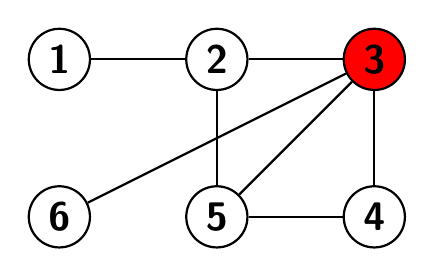
\begin{tikzpicture}[auto, node distance=2cm, every loop/.style={},
                    thick,main node/.style={circle,draw,font=\sffamily\Large\bfseries}]

  \node[main node] (1) {1};
  \node[main node] (2) [ right of=1] {2};
    \node[main node,fill=red] (3) [ right of=2] {3};
      \node[main node] (4) [ below of=3] {4};
        \node[main node] (5) [ left of=4] {5};
          \node[main node] (6) [ left of=5] {6};

\path[every node/.style={font=\sffamily\small}]
    (1) edge node [left] {} (2)
    (2) edge node [left] {} (3)
    (3) edge node [left] {} (4)
    (4) edge node [left] {} (5)
   
    (3) edge node [left] {} (5)
    (6) edge node [left] {} (3)
    (2) edge node [left] {} (5);
 
\end{tikzpicture}
\end{minipage}
}
\\
\\
\\
\noindent\fboxsep{%
\begin{minipage}{14em}
 \centering
 Step 3 \textbf{Optimal}
\begin{tikzpicture}[auto, node distance=2cm, every loop/.style={},
                    thick,main node/.style={circle,draw,font=\sffamily\Large\bfseries}]

  \node[main node] (1) {1};
  \node[main node,draw=none] (2) [ right of=1] {};
    \node[main node,draw=none] (3) [ right of=2] {};
      \node[main node,draw=none] (4) [ below of=3] {};
        \node[main node,draw=none] (5) [ left of=4] {};
          \node[main node,draw=none] (6) [ left of=5] {};
   
  
 
   

 
 
\end{tikzpicture}
\end{minipage}}%
\hfill%
\fboxsep{%
\begin{minipage}{14em}
 \centering
 Step 4 \textbf{Optimal}
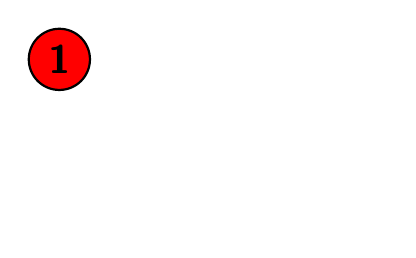
\begin{tikzpicture}[auto, node distance=2cm, every loop/.style={},
                    thick,main node/.style={circle,draw,font=\sffamily\Large\bfseries}]

   \node[main node,fill=red] (1) {1};
  \node[main node,draw=none] (2) [ right of=1] {};
    \node[main node,draw=none] (3) [ right of=2] {};
      \node[main node,draw=none] (4) [ below of=3] {};
        \node[main node,draw=none] (5) [ left of=4] {};
          \node[main node,draw=none] (6) [ left of=5] {};
   
\end{tikzpicture}
\end{minipage}
}

\\
\\
The Key these graph problems have seemed to always come when the algorithm reaches a tie. This is where the Algorithm can make mistakes.



\end{document}
 
 
\documentclass[11pt]{article}
\usepackage{tikz}
\usepackage{listings}
\usepackage[english]{babel}
\usepackage[autostyle]{csquotes}


\author{Andrew}
\date{text }

\begin{document}
\begin{center}
	CPSC 413 Assignment 1 \\
	by Andrew Garcia-Colrey
\end{center}
\part{Mailmen Problem}
Question 1
\begin{center}
	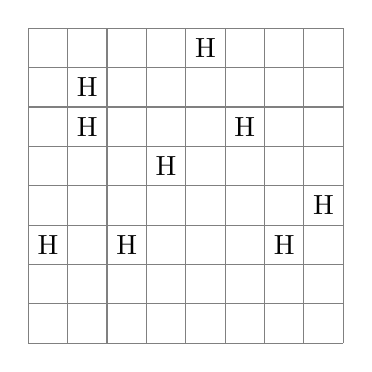
\begin{tikzpicture}
		\draw[step=0.5cm,color=gray] (-1,-1) grid (3,3);
		\node at (1.25,+2.75) {H};
		\node at (-.25,+2.25) {H};
		\node at (-0.25,+1.75) {H};
		\node at (+0.75,+1.25) {H};
		\node at (1.75,+1.75) {H};
		\node at (2.75,+0.75) {H};
		\node at (+2.25,0.25) {H};
		\node at (+.25,+0.25) {H};
		\node at (-.75,.25) {H};
	\end{tikzpicture}
\end{center}
Question 2
\hfill \break
\break
Two ways to look at this problem is to either minimize the amount of houses that are visited, or to maximize the amount of house each Mailmen finds. In my search for an algorithm I began debating between two main Algorithms I will refer to as \textbf{Shortest}  and \textbf{Most Houses}. 
\hfill \break
\break
\textbf{Shortest} simply starts by looking both down and right and checks to see from the current position of the mailman which one is closer and takes a step in that direction. then proceeds to checks again by looking down and to the right to see if there is a house closer to himself now that he has moved in on of the two directions.
\hfill \break
\break
\textbf{Most Houses} works in a similar fashion the previous Algorithm by looking in both directions. However where this Algorithm differ is that instead of looking for closest House, it instead looks for the most amount of Houses in that direction regardless of how far away it is. then upon moving in the direction with the most houses, the Algorithm then repeats the previous check by looking in both directions to ensure that.
\hfill \break
\break
However upon further examination and counter example exploration the  \textbf{Most Houses} fails to give an optimal solution for the following graph

\noindent\fboxsep{%
	\begin{minipage}{14em}
		\centering
		Figure 1 \textbf{Shortest}
		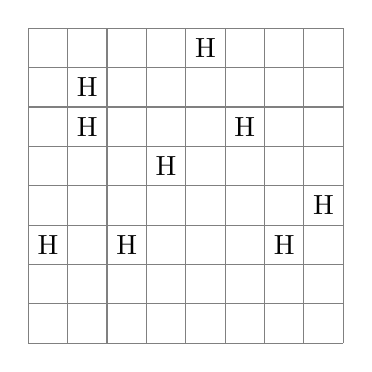
\begin{tikzpicture}
			
			\draw[step=0.5cm,color=gray] (-1,-1) grid (3,3);
			\node at (1.25,+2.75) {H};
			\node at (-.25,+2.25) {H};
			\node at (-0.25,+1.75) {H};
			\node at (+0.75,+1.25) {H};
			\node at (1.75,+1.75) {H};
			\node at (2.75,+0.75) {H};
			\node at (+2.25,0.25) {H};
			\node at (+.25,+0.25) {H};
			\node at (-.75,.25) {H};
		\end{tikzpicture}
	\end{minipage}}%
\hfill%
\fboxsep{%
	\begin{minipage}{14em}
		\centering
		Figure 2 \textbf{Most Houses}
		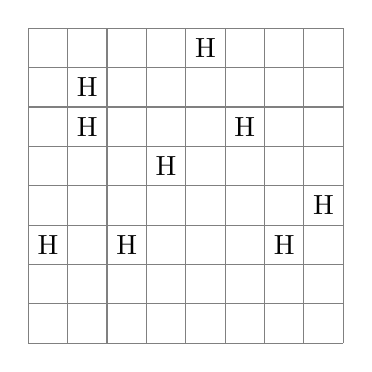
\begin{tikzpicture}
			
			\draw[step=0.5cm,color=gray] (-1,-1) grid (3,3);
			\node at (1.25,+2.75) {H};
			\node at (-.25,+2.25) {H};
			\node at (-0.25,+1.75) {H};
			\node at (+0.75,+1.25) {H};
			\node at (1.75,+1.75) {H};
			\node at (2.75,+0.75) {H};
			\node at (+2.25,0.25) {H};
			\node at (+.25,+0.25) {H};
			\node at (-.75,.25) {H};
		\end{tikzpicture}
	\end{minipage}
}





\hfill \break
\break
Where as the Shortest path method still gives the optimal number of paths which is 3. This does not mean that our  \textbf{Shortest} Algorithm is correct only that it is better then our \textbf{Most Houses} Algorithm.
\hfill \break
\break
\\
\newpage
\hfill \break
\break
AH = Array of tuple coordinates of Houses pre-sorted by y values
\newline
numberOfHouse = len(AH)
\newline
routes =  2D matrix with Mailmen as the first level and their routes as tuples as the inner array as tuples
\newline
currentRow = 0
\newline
currentCol = 0
\newline
numberOfMailMen = 0
\newline
N =  max number of rows and col in NxN matrix
\begin{lstlisting}
while(len(numberOfHouse) > 0)
    while (currentCol < N or currentRow < N):
            colIndex = (0,0)
            rowIndex = (0,0)
            for index to len(AH) :
                   if AH[index].0 == currentRow and rowIndex == (0,0):
                        rowIndex = AH[index]
                        continue
                   if AH[index].1 == currentCol and colIndex == (0,0) :
                        colIndex = AH[index]
                        continue
            deltaX =  rowIndex.0 - currentRow
            deltaY = colIndex.1 - currentCol
            if deltaX > deltaY:
                go down
                currentCol++
                routes[numberOfMailMen] = (currentRow,currentCol)
            if  deltaX < deltaY
                go right
                currentRow++
                routes[numberOfMailMen] = (currentRow,currentCol)
            for index to len(AH):
                if AH[index].0 == currentRow & AH[index].1 == currentCol:
                    numberOfHouse = numberOfHouse - 1
            if currentRow == (N-1) and currentRow == (N-1):
                numberOfMailMen = numberOfMailMen + 1
                currentCol = 0
                currentRow = 0
                
            



        
        
           
            
            
                
                
    
\end{lstlisting}
\\
\\
Not looking at the code above we will now look at the problem to try look for its complexity.
We are trying to find a algorithm that is poly-time. To do this we would like to show that in the worst case we are within the bounds of a poly-time complexity. 
\\
\\
\\
With this is mind let us look at the worst case where houses are on a reverse diagonal from our starting position.
\hfill \break
\break
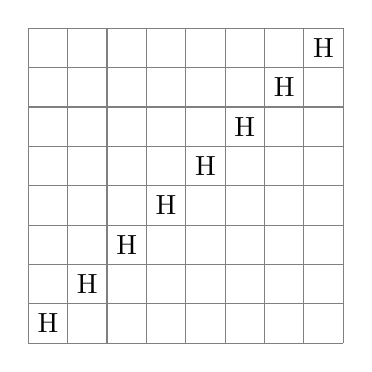
\begin{tikzpicture}
	
	\draw[step=0.5cm,color=gray] (-1,-1) grid (3,3);
	\node at (2.75,+2.75) {H};
	\node at (2.25,+2.25) {H};
	\node at (1.75,+1.75) {H};
	\node at (.75,+0.75) {H};
	\node at (+1.25,+1.25) {H};
	\node at (-.75,-.75) {H};
	\node at (+.25,+0.25) {H};
	\node at (-.25,-.25) {H};
\end{tikzpicture}
\hfill \break
\break
The above Grid showcases the worst case input for our algorithm. Where there is 8 house on the inverse diagonal from our starting positions (0,0). In this example we can clearly see that due to our Mailmens ability to only move down and to the right we will need at least N number of Mailmen to visit all of our houses. 
\hfill \break
\break
So in our worst case we need \textit{n} Mailmen for \textit{n} houses, in other words the number of Mailmen equals \textit{n}. Now each Mailman moves 2\textit{n}-1 spaces on his route. So this means that if we have the worst case input where the houses are on an inverse angle from our start position, we will need \textit{n} Mailmen who each move 2\textit{n}-1 times.
This gives us a complexity of \textit{n}(2\textit{n}-1), leading to a 2\textit{$n^2$} - \textit{n} which is in \textit{O($n^2$)}.

\hfill \break
\break
Now that we have the worst case run-time of an algorithm not including data structures or anything we need to keep track of let us look at the run-time of the algorithm above.

 


\pagebreak
\part{Marking Graphs}
Question 2.1
\\
For this question my solution is not the minimum amount of nodes that can be used to create a counter example. However I believe that the Graph that i have provided illustrates a key method and or insight into creating a counter example that provides an non-optimal solution.
\\
\\

\begin{center}
	
	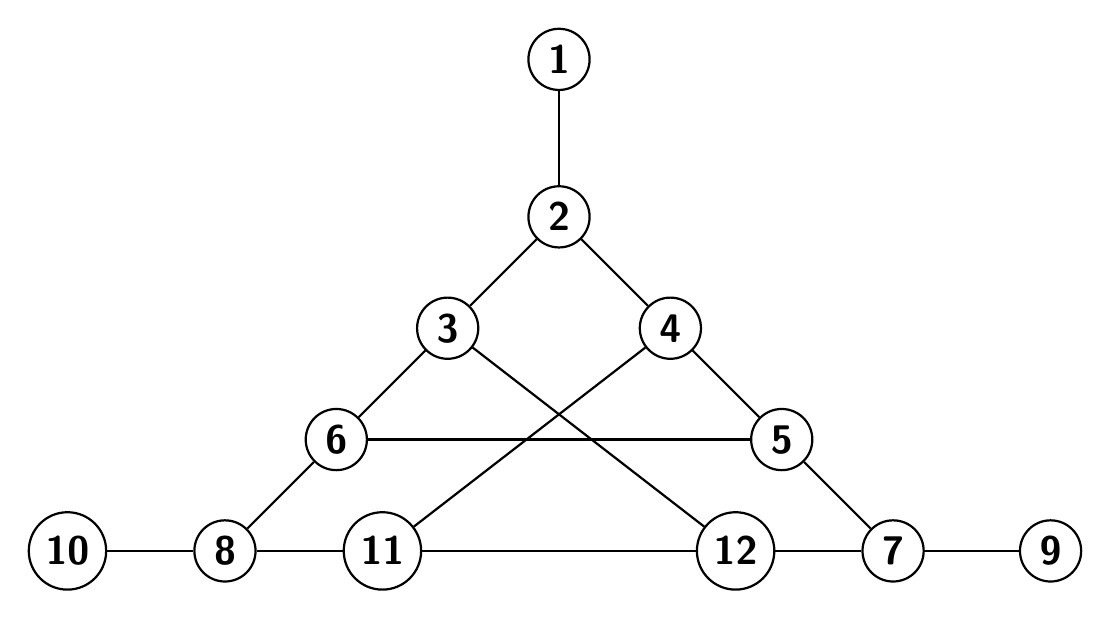
\begin{tikzpicture}[auto, node distance=2cm, every loop/.style={},
		thick,main node/.style={circle,draw,font=\sffamily\Large\bfseries}]
		
		\node[main node] (1) {1};
		\node[main node] (2) [below of=1] {2};
		\node[main node] (3) [below  left of=2] {3};
		\node[main node] (4) [below  right of=2] {4};
		\node[main node] (5) [below  right of=4] {5};
		\node[main node] (6) [below  left of=3] {6};
		\node[main node] (7) [below  right of=5] {7};
		\node[main node] (8) [below  left of=6] {8};
		\node[main node] (9) [  right of=7] {9};
		\node[main node] (10) [  left of=8] {10};
		\node[main node] (11) [  right of=8] {11};
		\node[main node] (12) [  left of=7] {12};
		         
		         
		\path[every node/.style={font=\sffamily\small}]
		(1) edge node [left] {} (2)
		(2) edge node [right] {} (4)
		(2) edge node [right] {} (3)
		(3) edge node [right] {} (6)
		(6) edge node [right] {} (8)
		(4) edge node [right] {} (5)
		(5) edge node [right] {} (7)
		(7) edge node [right] {} (9)
		(10) edge node [right] {} (8)
		(8) edge node [right] {} (11)
		(11) edge node [right] {} (12)
		(12) edge node [right] {} (7)
		(3) edge node [right] {} (12)
		(4) edge node [right] {} (11)
		(6) edge node [right] {} (5);
		    
		
	\end{tikzpicture}
\end{center}





\pagebreak
Question 2.2
\\
\\
The Graph I have given below is not the smallest number of nodes that you can use to give a counter example. In fact key to the counter example comes by denying the Algorithm an even edge and forcing it to pick an odd edge that is not going to give the Optimal Solution. The flaw with this algorithm like the one above comes from when there is a tie. particularly when there is no even Node to choose from and there by  \\\enquote{\textbf{mark[ing] any one vertex of odd degree}}.
\hfill \break
\break
\textbf{Non-optimal choice}
\begin{steps}
	\item \textbf{Step 1:} Start at Node 2 and \textbf{mark} it
	\item \textbf{Step 2:} Remove Node 2, 3 and 1 because they are now next to a \textbf{marked} Node
	\item \textbf{Step 3:} There are no Even Nodes so pick any Odd Node in this case\\ Node 4 and \textbf{mark} it
	\item \textbf{Step 4:} Remove Nodes 4 and 5 because they are now next to a \textbf{marked} Node
	\item \textbf{Step 5:} Now remaining Nodes 7 and 6 will need to be \textbf{marked} individually 
\end{steps}
\hfill \break




\noindent\fboxsep{%
	\begin{minipage}{14em}
		\centering
		Step 1 \textbf{non-optimal}
		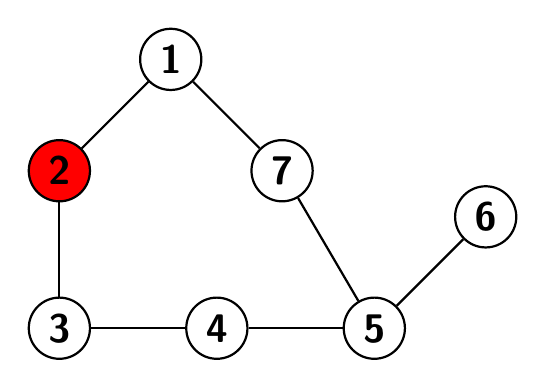
\begin{tikzpicture}[auto, node distance=2cm, every loop/.style={},
			thick,main node/.style={circle,draw,font=\sffamily\Large\bfseries}]
			
			\node[main node] (1) {1};
			\node[main node,fill=red] (2) [below left of=1] {2};
			\node[main node] (3) [below  of=2] {3};
			\node[main node] (4) [right  of=3] {4};
			\node[main node] (5) [ right  of=4] {5};
			\node[main node] (6) [above right  of=5] {6};
			\node[main node] (7) [below right  of=1] {7};
			
			
			\path[every node/.style={font=\sffamily\small}]
			(1) edge node [left] {} (2)
			(2) edge node [left] {} (3)
			(3) edge node [left] {} (4)
			(4) edge node [left] {} (5)
			(5) edge node [left] {} (6)
			(5) edge node [left] {} (7)
			(7) edge node [left] {} (1);
			 
		\end{tikzpicture}
	\end{minipage}}%
\hfill%
\fboxsep{%
	\begin{minipage}{14em}
		\centering
		Step 2 \textbf{non-optimal}
		\begin{tikzpicture}[auto, node distance=2cm, every loop/.style={},
			thick,main node/.style={circle,draw,font=\sffamily\Large\bfseries}]
			\node[main node,draw=none] (1) {};
			\node[main node,draw=none] (2) [below left of=1] {};
			\node[main node,draw=none] (3) [below  of=2] {};
			\node[main node] (4) [right  of=3] {4};
			\node[main node] (5) [ right  of=4] {5};
			\node[main node] (6) [above right  of=5] {6};
			\node[main node] (7) [below right  of=1] {7};
			
			
			\path[every node/.style={font=\sffamily\small}]
			  
			   
			   
			(4) edge node [left] {} (5)
			(5) edge node [left] {} (6)
			(5) edge node [left] {} (7)
			  
			 
		\end{tikzpicture}
	\end{minipage}
}
\hfill \break
\break


\noindent\fboxsep{%
	\begin{minipage}{14em}
		\centering
		Step 3 \textbf{non-optimal}
		\begin{tikzpicture}[auto, node distance=2cm, every loop/.style={},
			thick,main node/.style={circle,draw,font=\sffamily\Large\bfseries}]
			
			\node[main node,draw=none] (1) {};
			\node[main node,draw=none] (2) [below left of=1] {};
			\node[main node,draw=none] (3) [below  of=2] {};
			\node[main node,fill=red] (4) [right  of=3] {4};
			\node[main node] (5) [ right  of=4] {5};
			\node[main node] (6) [above right  of=5] {6};
			\node[main node] (7) [below right  of=1] {7};
			
			
			\path[every node/.style={font=\sffamily\small}]
			  
			   
			   
			(4) edge node [left] {} (5)
			(5) edge node [left] {} (6)
			(5) edge node [left] {} (7)
			   
			 
		\end{tikzpicture}
	\end{minipage}}%
\hfill%
\fboxsep{%
	\begin{minipage}{14em}
		\centering
		Step 4 \textbf{non-optimal}
		\begin{tikzpicture}[auto, node distance=2cm, every loop/.style={},
			thick,main node/.style={circle,draw,font=\sffamily\Large\bfseries}]
			\node[main node,draw=none] (1) {};
			\node[main node,draw=none] (2) [below left of=1] {};
			\node[main node,draw=none] (3) [below  of=2] {};
			\node[main node,draw=none] (4) [right  of=3] {};
			\node[main node,draw=none] (5) [ right  of=4] {};
			\node[main node] (6) [above right  of=5] {6};
			\node[main node] (7) [below right  of=1] {7};
			
			
			\path[every node/.style={font=\sffamily\small}]
			  
			   
			   
			 
			   
			 
		\end{tikzpicture}
	\end{minipage}
}

\begin{center}
	Step 5 \textbf{non-optimal}
	 
	\begin{tikzpicture}[auto, node distance=2cm, every loop/.style={},
		thick,main node/.style={circle,draw,font=\sffamily\Large\bfseries}]
		\node[main node,draw=none] (1) {};
		\node[main node,draw=none] (2) [below left of=1] {};
		\node[main node,draw=none] (3) [below  of=2] {};
		\node[main node,draw=none] (4) [right  of=3] {};
		\node[main node,draw=none] (5) [ right  of=4] {};
		\node[main node,fill=red] (6) [above right  of=5] {6};
		\node[main node,fill=red] (7) [below right  of=1] {7};
		
		
		\path[every node/.style={font=\sffamily\small}]
		  
		   
		   
		 
		   
		 
	\end{tikzpicture}
	\hfill \break
	This leads to four marked Nodes
	\hfill \break
	
\end{center}
\newpage
\hfill \break
\break
\textbf{Optimal choice}
\begin{steps}
	\item \textbf{Step 1:} Start at Node 2 and \textbf{mark} it
	\item \textbf{Step 2:} Remove Node 2, 3 and 1 because they are now next to a \textbf{marked} Node
	\item \textbf{Step 3:} Now \textbf{mark} 5
	\item \textbf{Step 4:} Remove Nodes 5, 4,7 and 6 because they are now next to a \textbf{marked} Node
\end{steps}
\hfill \break
\break

\noindent\fboxsep{%
	\begin{minipage}{14em}
		\centering
		Step 1 \textbf{Optimal}
		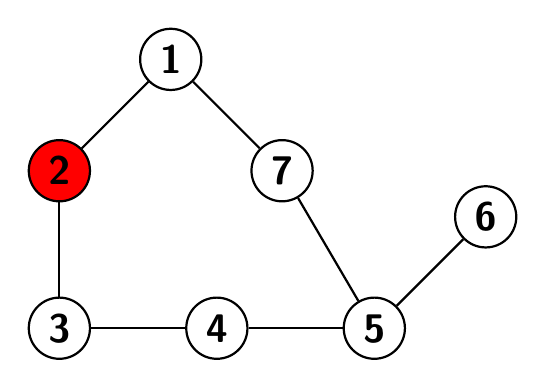
\begin{tikzpicture}[auto, node distance=2cm, every loop/.style={},
			thick,main node/.style={circle,draw,font=\sffamily\Large\bfseries}]
			
			\node[main node] (1) {1};
			\node[main node,fill=red] (2) [below left of=1] {2};
			\node[main node] (3) [below  of=2] {3};
			\node[main node] (4) [right  of=3] {4};
			\node[main node] (5) [ right  of=4] {5};
			\node[main node] (6) [above right  of=5] {6};
			\node[main node] (7) [below right  of=1] {7};
			
			
			\path[every node/.style={font=\sffamily\small}]
			(1) edge node [left] {} (2)
			(2) edge node [left] {} (3)
			(3) edge node [left] {} (4)
			(4) edge node [left] {} (5)
			(5) edge node [left] {} (6)
			(5) edge node [left] {} (7)
			(7) edge node [left] {} (1);
			 
		\end{tikzpicture}
	\end{minipage}}%
\hfill%
\fboxsep{%
	\begin{minipage}{14em}
		\centering
		Step 2 \textbf{Optimal}
		\begin{tikzpicture}[auto, node distance=2cm, every loop/.style={},
			thick,main node/.style={circle,draw,font=\sffamily\Large\bfseries}]
			\node[main node,draw=none] (1) {};
			\node[main node,draw=none] (2) [below left of=1] {};
			\node[main node,draw=none] (3) [below  of=2] {};
			\node[main node] (4) [right  of=3] {4};
			\node[main node] (5) [ right  of=4] {5};
			\node[main node] (6) [above right  of=5] {6};
			\node[main node] (7) [below right  of=1] {7};
			
			
			\path[every node/.style={font=\sffamily\small}]
			  
			   
			   
			(4) edge node [left] {} (5)
			(5) edge node [left] {} (6)
			(5) edge node [left] {} (7)
			  
			 
		\end{tikzpicture}
	\end{minipage}
}
\hfill \break
\break


\noindent\fboxsep{%
	\begin{minipage}{14em}
		\centering
		Step 3 \textbf{Optimal}
		\begin{tikzpicture}[auto, node distance=2cm, every loop/.style={},
			thick,main node/.style={circle,draw,font=\sffamily\Large\bfseries}]
			
			\node[main node,draw=none] (1) {};
			\node[main node,draw=none] (2) [below left of=1] {};
			\node[main node,draw=none] (3) [below  of=2] {};
			\node[main node] (4) [right  of=3] {4};
			\node[main node,fill=red] (5) [ right  of=4] {5};
			\node[main node] (6) [above right  of=5] {6};
			\node[main node] (7) [below right  of=1] {7};
			
			
			\path[every node/.style={font=\sffamily\small}]
			  
			   
			   
			(4) edge node [left] {} (5)
			(5) edge node [left] {} (6)
			(5) edge node [left] {} (7)
			   
			 
		\end{tikzpicture}
	\end{minipage}}%
\hfill%
\fboxsep{%
	\begin{minipage}{14em}
		\centering
		Step 4 \textbf{Optimal}
		\begin{tikzpicture}[auto, node distance=2cm, every loop/.style={},
			thick,main node/.style={circle,draw,font=\sffamily\Large\bfseries}]
			\node[main node,draw=none] (1) {};
			\node[main node,draw=none] (2) [below left of=1] {};
			\node[main node,draw=none] (3) [below  of=2] {};
			\node[main node,draw=none] (4) [right  of=3] {};
			\node[main node,draw=none] (5) [ right  of=4] {};
			\node[main node,draw=none] (6) [above right  of=5] {};
			\node[main node,draw=none] (7) [below right  of=1] {};
			
			
			\path[every node/.style={font=\sffamily\small}]
			  
			   
			   
			 
			   
			 
		\end{tikzpicture}
	\end{minipage}
}
\hfill \break
\break

This leads to two \textbf{Marked} Nodes
\hfill \break
\break























\pagebreak
\hfill \break
\break
Question 2.3
\hfill \break
\break
This question was by far the more difficult of all three. How I decided to tackle the problem was to control the entry points by which the Algorithm could enter the graph. So I created a graph with only two entry points both with the least degree. One of the entry points would give the optimal solution while the other would give the a satisfactory solution but not optimal.
\hfill \break
\break
\textbf{Non-optimal choice}
\begin{steps}
	\item \textbf{Step 1:} Start at Node 1
	\item \textbf{Step 2:} Move to Node 2 because it has a Degree of 3 and \textbf{mark} it
	\item \textbf{Step 3:} Remove Node 1, 5 and 3 because they are now next to a \textbf{marked} Node
	\item \textbf{Step 4:} Only Nodes left are 6 and 4 which are not connected by and edge so they each must be marked themselves
\end{steps}
\hfill \break
\break
This leads to three marked Nodes
\begin{center}
	
\end{center}
\noindent\fboxsep{%
	\begin{minipage}{14em}
		\centering
		Step 1 \textbf{non-optimal}
		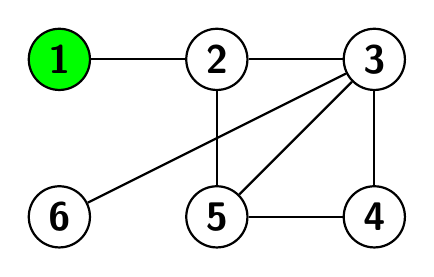
\begin{tikzpicture}[auto, node distance=2cm, every loop/.style={},
			thick,main node/.style={circle,draw,font=\sffamily\Large\bfseries}]
			
			\node[main node,fill=green] (1) {1};
			\node[main node] (2) [ right of=1] {2};
			\node[main node] (3) [ right of=2] {3};
			\node[main node] (4) [ below of=3] {4};
			\node[main node] (5) [ left of=4] {5};
			\node[main node] (6) [ left of=5] {6};
			
			\path[every node/.style={font=\sffamily\small}]
			(1) edge node [left] {} (2)
			(2) edge node [left] {} (3)
			(3) edge node [left] {} (4)
			(4) edge node [left] {} (5)
			   
			(3) edge node [left] {} (5)
			(6) edge node [left] {} (3)
			(2) edge node [left] {} (5);
			 
		\end{tikzpicture}
	\end{minipage}}%
\hfill%
\fboxsep{%
	\begin{minipage}{14em}
		\centering
		Step 2 \textbf{non-optimal}
		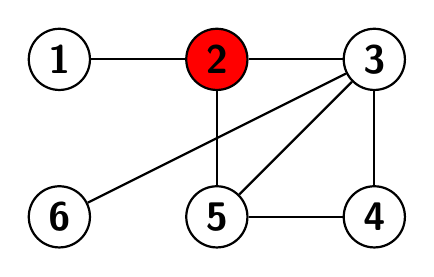
\begin{tikzpicture}[auto, node distance=2cm, every loop/.style={},
			thick,main node/.style={circle,draw,font=\sffamily\Large\bfseries}]
			
			\node[main node] (1) {1};
			\node[main node,fill=red] (2) [ right of=1] {2};
			\node[main node] (3) [ right of=2] {3};
			\node[main node] (4) [ below of=3] {4};
			\node[main node] (5) [ left of=4] {5};
			\node[main node] (6) [ left of=5] {6};
			
			\path[every node/.style={font=\sffamily\small}]
			(1) edge node [left] {} (2)
			(2) edge node [left] {} (3)
			(3) edge node [left] {} (4)
			(4) edge node [left] {} (5)
			   
			(3) edge node [left] {} (5)
			(6) edge node [left] {} (3)
			(2) edge node [left] {} (5);
			 
		\end{tikzpicture}
	\end{minipage}
}
\\
\\
\\
\noindent\fboxsep{%
	\begin{minipage}{14em}
		\centering
		 
		Step 3 \textbf{non-optimal}
		\begin{tikzpicture}[auto, node distance=2cm, every loop/.style={},
			thick,main node/.style={circle,draw,font=\sffamily\Large\bfseries}]
			
			\node[main node,draw=none] (1) {};
			\node[main node,draw=none] (2) [ right of=1] {};
			\node[main node,draw=none] (3) [ right of=2] {};
			\node[main node] (4) [ below of=3] {4};
			\node[main node,draw=none] (5) [ left of=4] {};
			\node[main node] (6) [ left of=5] {6};
			
			
			    
			    
			   
			    
			  
			
			 
		\end{tikzpicture}
	\end{minipage}}%
\hfill%
\fboxsep{%
	\begin{minipage}{14em}
		\centering
		Step 4 \textbf{non-optimal}
		\begin{tikzpicture}[auto, node distance=2cm, every loop/.style={},
			thick,main node/.style={circle,draw,font=\sffamily\Large\bfseries}]
			
			\node[main node,draw=none] (1) {};
			\node[main node,draw=none] (2) [ right of=1] {};
			\node[main node,draw=none] (3) [ right of=2] {};
			\node[main node,fill=red] (4) [ below of=3] {4};
			\node[main node,draw=none] (5) [ left of=4] {};
			\node[main node,fill=red] (6) [ left of=5] {6};
			 
		\end{tikzpicture}
	\end{minipage}
}

\pagebreak
\hfill \break
\break
\textbf{Optimal choice}
\begin{steps}
	\item \textbf{Step 1:} Start at Node 6
	\item \textbf{Step 2:} Move to Node 3 because it has a Degree of 4 and \textbf{mark} it
	\item \textbf{Step 3:} Remove Node 3, 5, 2 and 4 because they are now next to a \textbf{marked} Node
	\item \textbf{Step 4:} Only Node left is 1 and must be \textbf{marked} itself
\end{steps}
\hfill \break
\break
This leads to only two marked Nodes being needed and is the Optimal Solution for this Graph

\begin{center}
	
\end{center}
\noindent\fboxsep{%
	\begin{minipage}{14em}
		\centering
		Step 1 \textbf{Optimal}
		\begin{tikzpicture}[auto, node distance=2cm, every loop/.style={},
			thick,main node/.style={circle,draw,font=\sffamily\Large\bfseries}]
			
			\node[main node] (1) {1};
			\node[main node] (2) [ right of=1] {2};
			\node[main node] (3) [ right of=2] {3};
			\node[main node] (4) [ below of=3] {4};
			\node[main node] (5) [ left of=4] {5};
			\node[main node,fill=green] (6) [ left of=5] {6};
			
			\path[every node/.style={font=\sffamily\small}]
			(1) edge node [left] {} (2)
			(2) edge node [left] {} (3)
			(3) edge node [left] {} (4)
			(4) edge node [left] {} (5)
			   
			(3) edge node [left] {} (5)
			(6) edge node [left] {} (3)
			(2) edge node [left] {} (5);
			 
		\end{tikzpicture}
	\end{minipage}}%
\hfill%
\fboxsep{%
	\begin{minipage}{14em}
		\centering
		Step 2 \textbf{Optimal}
		\begin{tikzpicture}[auto, node distance=2cm, every loop/.style={},
			thick,main node/.style={circle,draw,font=\sffamily\Large\bfseries}]
			
			\node[main node] (1) {1};
			\node[main node] (2) [ right of=1] {2};
			\node[main node,fill=red] (3) [ right of=2] {3};
			\node[main node] (4) [ below of=3] {4};
			\node[main node] (5) [ left of=4] {5};
			\node[main node] (6) [ left of=5] {6};
			
			\path[every node/.style={font=\sffamily\small}]
			(1) edge node [left] {} (2)
			(2) edge node [left] {} (3)
			(3) edge node [left] {} (4)
			(4) edge node [left] {} (5)
			   
			(3) edge node [left] {} (5)
			(6) edge node [left] {} (3)
			(2) edge node [left] {} (5);
			 
		\end{tikzpicture}
	\end{minipage}
}
\\
\\
\\
\noindent\fboxsep{%
	\begin{minipage}{14em}
		\centering
		Step 3 \textbf{Optimal}
		\begin{tikzpicture}[auto, node distance=2cm, every loop/.style={},
			thick,main node/.style={circle,draw,font=\sffamily\Large\bfseries}]
			
			\node[main node] (1) {1};
			\node[main node,draw=none] (2) [ right of=1] {};
			\node[main node,draw=none] (3) [ right of=2] {};
			\node[main node,draw=none] (4) [ below of=3] {};
			\node[main node,draw=none] (5) [ left of=4] {};
			\node[main node,draw=none] (6) [ left of=5] {};
			   
			  
			 
			   
			
			 
			 
		\end{tikzpicture}
	\end{minipage}}%
\hfill%
\fboxsep{%
	\begin{minipage}{14em}
		\centering
		Step 4 \textbf{Optimal}
		\begin{tikzpicture}[auto, node distance=2cm, every loop/.style={},
			thick,main node/.style={circle,draw,font=\sffamily\Large\bfseries}]
			
			\node[main node,fill=red] (1) {1};
			\node[main node,draw=none] (2) [ right of=1] {};
			\node[main node,draw=none] (3) [ right of=2] {};
			\node[main node,draw=none] (4) [ below of=3] {};
			\node[main node,draw=none] (5) [ left of=4] {};
			\node[main node,draw=none] (6) [ left of=5] {};
			   
		\end{tikzpicture}
	\end{minipage}
}

\\
\\
The Key these graph problems have seemed to always come when the algorithm reaches a tie. This is where the Algorithm can make mistakes.



\end{document}